\documentclass[10pt,conference,compsocconf]{IEEEtran}

\usepackage{hyperref}
\usepackage{graphicx}	% For figure environment


\begin{document}
\title{Pattern Classification \& Machine Learning - Project 1 \\ \textit{Finding the Higgs Boson}}

\author{
  Apolline Lafarge, Lo{\"i}c Ottet, Dimitrios Sarigiannis\\
  \textit{Department of Computer Science, EPFL Lausanne, Switzerland}
}

\maketitle

\begin{abstract}
In this report, we summarize our findings for the first project of the machine learning course taught at the EPFL. The goal of the project is the computation as well as the error estimation of predictions of a classification dataset of the CERN Higgs boson. Key aspects of the project are exploratory data analysis, feature processing, the implementation of several regression and classification machine learning methods and the comparison of different models using cross-validation.
\end{abstract}

\section*{Introduction}
The problem that we are asked to solve is about classifying particles into two clases: {Higgs boson, Other} . More specifically, we are facing a binary classification problem and given a huge dataset which we need to use for training our models, we need to apply both regression and classification methods.
Further analysis and plots can be found on  \verb|project1.ipynb|
\section{Data Analysis \& Processing}
In this section, we perform a data analysis on the given dataset and we describe our preprocessing steps.
\subsection{Data Description}
Our dataset consists of 250000 particles and each particle has a binary class {s=1,b=-1} which represents its type and 30 more features. By visualizing a simple plot, we realize that the classes in the dataset are skewed, having approximately 160000 particles in class b and 90000 particles in class s. Also, by visualizing each feature with respect to its corresponding output we searched for features that give us zero profit in predicting the class of the particle. However, none of the features could be eliminated for sure (since we do not know what these features represent in reality). All the aforementioned plots can be seen in our notebook project.
\subsection{Rank Deficiency}
By running \verb|matrix_rank()| function of numpy library we manage to get the rank of our training data. Because the rank of this matrix is 30 (our columns-features are also 30) we claim that our data are not ill-conditioned meaning that they are not linearly depend to each other. As we can see later, since we have a very good rank on our training data set, we expect to get very good score in Least Squares using normal equations method.
\subsection{Standardization}
We applied standardization on the training and test datasets before doing any further work. In addition to reducing the data on each feature to zero mean and unit variance as was done in the provided standardization function, we also handled the values which could not be measured (those with value -999) by replacing them by the mean value of their feature. The mean was of course calculated without including these outliers.
\subsection{Feature Elimination}
Some features are more important than others to the model accuracy. So, we tried to get an evaluation of the importance of each feature. In order to do this, we computed the feature's usefulness by their correlation with the class labels y. We obtain the graph below in figure1 (where a coefficient near from 1 or -1 traduces an high correlation, and 0 no correlation) :

\begin{figure}[h]
  \centering
  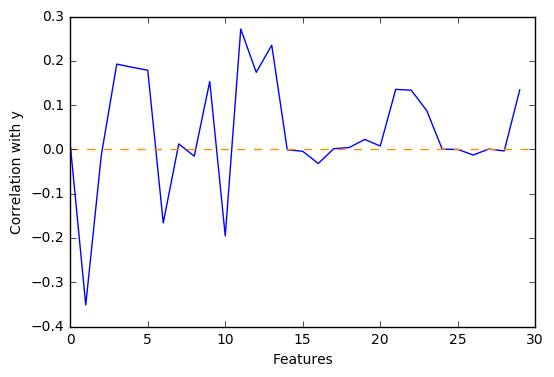
\includegraphics[width=0.42\columnwidth]{features}
  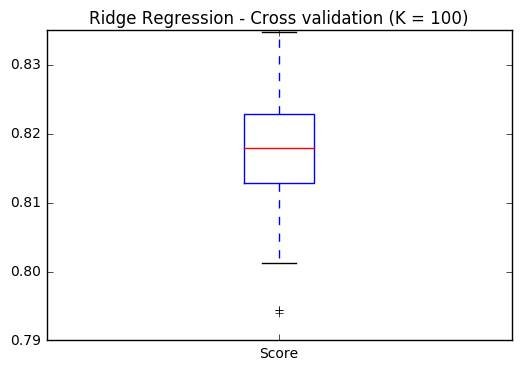
\includegraphics[width=0.42\columnwidth]{boxplot}
  \caption{left: feature's correlation with y, right:score boxplot}
  \vspace{-3mm}
\end{figure}

Then, we only choose a threshold (in absolute value) above which we keep the features. In our case, we observe feature selection does’nt enable to get better results. However, it is possible to get similar results with fewer features which actually makes our computations cheaper.
\subsection{Quadradic space}
We managed to compute quadratic decision boundaries. However, this method push us to handle a lot of features ($D(D+3)/2$ where $D$ is the number of features). Of course, we could not manipulate this in a reasonable time, then we proceeded to feature selection before transforming the data.
As we got better results using other models, we didn’t keep this solution. A concrete example is given in the code.
\subsection{Polynomial expansion}
The main feature selection process we ended up using for the project is based on polynomial basis functions. In order to put more weight on more significant features, we added successive powers of each feature to the dataset, up to a certain degree that we deemed optimal.
The way we selected the optimal degree for each feature was the following: for each feature in turn, we added to the original dataset polynomial expansions of the examined feature, up to a certain predefined maximal degree. Then we chose the best degree based on the results the partial expansion gave us.
Knowing the best degree for each of the individual features, we then built our final dataset by adding the optimal number of polynomial expansion for each feature in turn. During that step, some features for which the optimal degree we obtained was 0 were plainly deleted from the dataset, thereby achieving a similar result as feature elimination would have.

\section{ML Methods}
In this section we perfom an analysis on our implemented Machine Learning Regression and Classification Methods. Before doing that, we also need to mention how we performed our model selection.
\subsection{Model Selection}
Once our dataset was ready, we then proceeded to find the method yielding the best results for our dataset. To do so, we selected several potential values for the various parameters of the regression and classification methods. We ran this step only on the $\gamma$ and $\lambda$, as the initial weight vector doesn't seem to play a significant role and the number of iterations has no "optimal" value as it represents only a tradeoff between result precision and running time.
\par In order to avoid overfitting on our training data, we implemented 5-fold cross validation to obtain an unbiased estimate of the obtained score, and that way the best method and parameter selection for our task. In our code, the \verb|cross_validation()| function is a generic one which is called by each of the \verb|test_##| functions based on the method we wanted to test.

\subsection{ML Regression Methods}
For applying regression, we have implemented the following methods:
\subsubsection{Least Squares using Gradient Descent}
The crucial aspect of this method is the choice of the step-size $\gamma$ and the choice of the convergence criterion. Ideally, we should select a step-size $\gamma$ that minimizes $min f(x_k - \gamma \nabla f(x_k))$ with $\gamma>0$ and $k$ being the iteration number. However, this computation is very expensive and we rather choose an non-optimal step-size easier to compute. We finally choose a $\gamma$ for which we observe fast convergence on our dataset. We could also have set a threshold (i.e $10^{-5}$) in order to find out where we should stop iterating but this was not necessary for this project.

\subsubsection{Least Squares using Stochastic Gradient Descent}
The same aforementioned statements are also true for stochastic gradient descent. The only difference now is that we now pick only one random point at each iteration and thus we might let the algorithm do more iterations until it converges. Since the computational cost is much cheaper now, even when we do more iterations we get a faster convergence .
\subsubsection{Least Squares using normal equations}
Given that the input matrix X is not ill-conditioned, we are able to apply least squares using normal equations. Least squares is going to give us the final w parameters really fast, and we also expect to get good score because of the linear independence of the features. Indeed, we managed to take a very high score of 0.81 by using polynomial degree of 12.
\subsubsection{Ridge Regression using normal equations}
Ridge regression is a "normalized" least squares and we expected to get the same good results as least squares. Indeed, we got a bit better score from least squares with a lambda close to 0 ($10^{-6}$) meaning that these two methods are almost equal. The most important aspect of ridge regression is the choice of $\lambda$ which was found by cross validation. We varied the value of $\lambda$ from $10^{-9}$ to $10^{3}$, choosing a total of 200 points in between and chose then the $\lambda$ resulting in the smallest averaged test RMSE.

\subsection{ML Classification Methods}
For applying classification, we have implemented the following methods:
\subsubsection{Logistic Regression using Gradient Descent}
Our implementation can do a descent classification for small datasets, but for the given dataset we face some numerical issues due to the very big values that are created during the process.
\subsubsection{Regularized Logistic Regression using Gradient Descent}
The same problem occurs in that function as well. However, if we could overcome the numerical issues we would expect to get a slightly better score than ridge regression.

\section{Performance Analysis}
In this report, we analyzed a binary classification dataset with both regression and classification methods. The data preperation and preprocessing played a crucial role in order to get good results. For the regression methods, we got our best score (0.81396) from Ridge Regression ($\lambda$=1e-06) which was expected since the columns-features of our dataset were totally not linearly depend. Also, the lambda was pretty small meaning that least squares is also a good method and almost equal to ridge regression. For the classification methods, we were expected to get slightly better results than the regression methods but since we had some numerical issues in our implementation, we did not manage to do so.

%\bibliographystyle{IEEEtran}
%\bibliography{literature}

\end{document}
